\documentclass{beamer}
% --- add to your preamble ---
\usepackage{pgfplots}
\pgfplotsset{compat=1.18}
\definecolor{matchblue}{HTML}{2A78D6}
\definecolor{dimline}{HTML}{C3C2B7}
\definecolor{axisgray}{HTML}{898781}
\definecolor{inkmuted}{HTML}{52514E}
\definecolor{efffill}{HTML}{D6EBDF}
\definecolor{inefffill}{HTML}{FBDCCB}
\pgfplotsset{
  effband/.style={fill=efffill},
  ineffband/.style={fill=inefffill},
  matchline/.style={draw=matchblue, line width=1.6pt, line join=round, mark=none},
  satline/.style={draw=inkmuted, line width=0.6pt, dashed, mark=none},
}
\tikzset{regimelabel/.style={font=\small\bfseries, text=inkmuted}}

% placeholders for the paper's macros (drop these in your deck)
\providecommand{\opt}{\star}
\providecommand{\Th}{T_h}
\providecommand{\effmatchings}{\mathcal{T}^{\mathrm{eff}}}
\begin{document}
% --- the frame ---
\begin{frame}{When does the platform match the high types?}
  \centering
  % generated by make_prop_regimes.py from results/exp_13/star (instance #1, linear costs)
% overlays: <1> the sweep; <2>-<5> regimes (ii)-(v); <6> all regimes
\begin{tikzpicture}
\begin{axis}[
  width=0.78\linewidth, height=0.28\textheight, scale only axis,
  xmin=3.4, xmax=8.0, ymin=-0.1, ymax=1.1,
  axis lines=left, axis line style={draw=axisgray, -}, tick style={draw=axisgray},
  ytick={0,1}, yticklabels={none, all}, ylabel={high types matched},
  xtick={4.4,6.6,7.26},
  xticklabels={$\epsilon_h^-$, $\epsilon_h^+$, $\underline{\epsilon}_h$},
  xlabel={$\epsilon_h$}, xlabel style={at={(ticklabel* cs:1)}, anchor=north west},
  ticklabel style={font=\small}, label style={font=\small}, typeset ticklabels with strut,
  clip=false,
]
% regime bands
\only<2,6>{\addplot[effband, draw=none, forget plot] coordinates {(3.4,-0.1) (3.4,1.1) (4.4,1.1) (4.4,-0.1)} \closedcycle; \addplot[effband, draw=none, forget plot] coordinates {(6.6,-0.1) (6.6,1.1) (7,1.1) (7,-0.1)} \closedcycle;}
\only<3,6>{\addplot[ineffband, draw=none, forget plot] coordinates {(4.4,-0.1) (4.4,1.1) (6.6,1.1) (6.6,-0.1)} \closedcycle;}
\only<4,6>{\addplot[effband, draw=none, forget plot] coordinates {(7,-0.1) (7,1.1) (7.26,1.1) (7.26,-0.1)} \closedcycle;}
\only<5,6>{\addplot[ineffband, draw=none, forget plot] coordinates {(7.26,-0.1) (7.26,1.1) (8,1.1) (8,-0.1)} \closedcycle;}
% saturation threshold n_h + eps_h = K
\addplot[satline, forget plot] coordinates {(7,-0.1) (7,1.1)};
\node[font=\scriptsize, text=inkmuted, anchor=south east] at (axis cs:7,1.1) {$n_h+\epsilon_h\le K$};
\node[font=\scriptsize, text=inkmuted, anchor=south west] at (axis cs:7,1.1) {$>K$};
% the observed sweep: full line on <1> and <6>, dimmed with the current regime highlighted on <2>-<5>
\only<1,6>{\addplot[matchline] coordinates {(3.4,0) (4.4125,0) (4.4125,1) (6.5875,1) (6.5875,0) (7.2662,0) (7.2662,1) (8,1)};}
\only<2-5>{\addplot[matchline, draw=dimline] coordinates {(3.4,0) (4.4125,0) (4.4125,1) (6.5875,1) (6.5875,0) (7.2662,0) (7.2662,1) (8,1)};}
\only<2>{\addplot[matchline] coordinates {(3.4,0) (4.4,0)}; \addplot[matchline] coordinates {(6.6,0) (7,0)};}
\only<3>{\addplot[matchline] coordinates {(4.4,0) (4.4125,0) (4.4125,1) (6.5875,1) (6.5875,0) (6.6,0)};}
\only<4>{\addplot[matchline] coordinates {(7,0) (7.26,0)};}
\only<5>{\addplot[matchline] coordinates {(7.26,0) (7.2662,0) (7.2662,1) (8,1)};}
% regime numerals, centred in each band
\only<2,6>{\node[regimelabel] at (axis cs:3.9,0.5) {(ii)}; \node[regimelabel, font=\footnotesize\bfseries] at (axis cs:6.8,0.62) {(ii)};}
\only<3,6>{\node[regimelabel] at (axis cs:5.5,0.5) {(iii)};}
\only<4,6>{\node[regimelabel, font=\footnotesize\bfseries] at (axis cs:7.13,0.38) {(iv)};}
\only<5,6>{\node[regimelabel] at (axis cs:7.63,0.5) {(v)};}
\end{axis}
\end{tikzpicture}


  \vspace{0.6em}
  \small
  \begin{minipage}[t][2.6em]{0.95\linewidth}\centering
  \only<1>{Star costs, instance \#1: share of high types matched as $\epsilon_h$ grows.}
  \only<2>{\textbf{(ii)} $n_h+\epsilon_h\le K$, $\epsilon_h\notin(\epsilon_h^-,\epsilon_h^+)$: optimal matchings are $\effmatchings$, $\Pi^\opt=A-B_\ell$.}
  \only<3>{\textbf{(iii)} $n_h+\epsilon_h\le K$, $\epsilon_h\in(\epsilon_h^-,\epsilon_h^+)$: $\Th\subseteq T^\opt\notin\effmatchings$, $\Pi^\opt=A-B_h$.}
  \only<4>{\textbf{(iv)} $n_h+\epsilon_h>K$, $\epsilon_h\le\underline{\epsilon}_h$: optimal matchings are $\effmatchings$, $\Pi^\opt=A-B_\ell$.}
  \only<5>{\textbf{(v)} $n_h+\epsilon_h>K$, $\epsilon_h>\underline{\epsilon}_h$: $\Th\subseteq T^\opt\notin\effmatchings$, $\Pi^\opt=A-B_h$.}
  \only<6>{\colorbox{efffill}{efficient: $\Pi^\opt=A-B_\ell$} \quad \colorbox{inefffill}{inefficient: $\Pi^\opt=A-B_h$}}
  \end{minipage}
\end{frame}
\end{document}
